\documentclass[letterpaper, 10 pt, conference]{ieeeconf} 

\usepackage[utf8]{inputenc}
\usepackage[T1]{fontenc}
\usepackage{amsmath,amssymb,amsfonts}
\usepackage{graphicx}
\usepackage{booktabs}
\usepackage{hyperref}
\usepackage{tikz}
\usetikzlibrary{arrows.meta, positioning, shapes.geometric, fit, calc}
\usepackage{algorithm}
\usepackage{algpseudocode}
\usepackage{cite}
\usepackage{caption}
\usepackage{subcaption}
\usepackage{graphicx}
\usepackage{xcolor}
\usepackage{enumitem}
\usepackage{multirow}
\usepackage[normalem]{ulem}
\usepackage{amsfonts}
\usepackage[bbgreekl]{mathbbol}
\DeclareSymbolFontAlphabet{\mathbbm}{bbold}
\DeclareSymbolFontAlphabet{\mathbb}{AMSb}%
\usepackage{bm}
\usepackage{amsthm}
\newtheorem{theorem}{Theorem}
\newtheorem{problem}{Problem}
\newtheorem{definition}{Definition}
\newtheorem{remark}{Remark}
\newtheorem{lemma}{Lemma}
\newtheorem{result}{Result}
\newtheorem{assumption}{Assumption}
\usepackage[title]{appendix}%
\IEEEoverridecommandlockouts



\begin{document}

\title{\LARGE \bf Closed-Loop Control of Symbolic Music Generation\\via Group Relative Policy Optimization}







%\author{
%\IEEEauthorblockN{Aditya Kinjawadekar}
%\IEEEauthorblockA{Department of Electronics and %Communication Engineering}
%}



\author{Aditya Kinjawadekar$^{a}$, Midhun T. Augustine$^{b}$,  
Surender Kannaiyan$^{a}$, Dibyajyoti Baidya$^{c}$  
\thanks{$^a$ Department of Electronics and Communication Engineering,   Visvesvaraya National Institute of Technology,  Nagpur, India, 440 010. \newline
$^b$ Department of Chemical and Materials Engineering, University of Alberta, Edmonton, Canada, T6G 2R3. \newline
$^c$ Department of Chemical  Engineering, Indian Institute of Technology Bombay, Mumbai, India, 400 076.
}}

\maketitle

% ═══════════════════════════════════════════════════════════════
\begin{abstract}
This paper presents a closed-loop control framework for symbolic music generation that integrates reinforcement learning (RL) with principles from control theory. Specifically, symbolic music generation is formulated as a \emph{feedback control} problem in which a causal Transformer operating over compound word (CP) token states serves as the \emph{plant}, a pretrained MidiBERT-based reward model functions as the \emph{sensor} by providing scalar quality assessments of the generated sequences, and a group relative policy optimization (GRPO) algorithm acts as the \emph{controller}, updating the policy to optimize the quality of the generated musical pieces.
Kullback-Leibler (KL) divergence regularization with respect to a frozen reference policy serves as a Lyapunov-like stability constraint, bounding policy drift within a trust region. An entropy floor acts as an exploration-preserving regularizer, preventing premature collapse of the action distribution and maintaining policy diversity. The proposed framework is trained on the ATEPP classical piano corpus (approximately 14,000 CP sequences) and fine-tuned using 1,500 GRPO optimization steps. Experimental results demonstrate a monotonic improvement in the evaluation reward while maintaining bounded KL divergence. These findings support the proposed control-theoretic interpretation and indicate that principles from optimal and adaptive control can provide a systematic and theoretically grounded framework for improving RL-based symbolic music generation.
\end{abstract}

% \begin{IEEEkeywords}
% Feedback control, Policy optimization, Reinforcement learning, Symbolic music generation, Lyapunov stability, Trust region methods
% \end{IEEEkeywords}

% ═══════════════════════════════════════════════════════════════
\section{Introduction}
Algorithmic composition is an active area of research focused on the automated generation of music using mathematical or computational models \cite{Nierhaus2009}. Approaches in this field are based on autoregressive models \cite{Yu2026,Nierhaus2009}, probabilistic models \cite{Allan2004}, rule-based systems \cite{Boenn2010,Anders2012},  deep learning (DL) models \cite{Briot2020}, among others.  Autoregressive generative models for symbolic music produce locally coherent sequences but lack mechanisms for global quality assurance, a problem analogous to open-loop control of nonlinear dynamical systems. Similarly, Markov chains, probabilistic models, and other initial approaches typically generate music in an open-loop manner, without explicit mechanisms for enforcing long-range consistency \cite{Allan2004,Loy2006}.
%\sout{Autoregressive Transformers trained via maximum likelihood estimation (MLE) on symbolic music corpora generate sequences by iterating a learned one-step transition map. This paradigm is inherently \emph{open-loop}: the generator commits to a distribution $p_{\bm{\theta}}(\textbf{x}_{t+1} \mid \textbf{x}_{\le t})$ without any feedback from an external quality criterion}.
Open-loop policies are inherently sensitive and may lead to unstable predictions; small prediction errors accumulate over a long generation horizon, leading to mode collapse, repetitive motifs, or structural incoherence~\cite{Astrom2008,holtzman2020curious}.

In control theory, the standard approach to addressing the limitations of open-loop systems is to incorporate \emph{feedback} \cite{Astrom2008}. In a feedback control system, a sensor measures the system output, the measured output is compared with a reference signal, and a controller adjusts the system input to minimize the tracking error.
Reinforcement learning (RL) is a data-driven feedback control approach that learns closed-loop policies through interaction with an environment or system. More recently, RL has been applied to symbolic music generation \cite{Jaques2016,Kotecha2018,dadman2023,dadman2024,cideron2024,Justus2023}, due to its ability to incorporate music quality-related measures into the reward function. For example, \cite{Jaques2016} introduced an RL-based framework that fine-tunes a recurrent neural network using policy optimization to improve sequence generation while retaining the knowledge learned during supervised pre-training. This approach has demonstrated effectiveness in applications such as symbolic music generation and computational molecular generation.  In addition, several studies have investigated the use of RL for symbolic music generation, exploring topics such as multi-agent RL, user-guided composition, and alignment with human preferences \cite{Kotecha2018,dadman2023,dadman2024,cideron2024}. In a similar direction, \cite{Justus2023} proposed a human-in-the-loop RL framework that incorporates human feedback into the training process, enabling the generation of music that better aligns with user preferences and subjective notions of musical quality. In addition, Transformer-based architectures have been widely adopted for symbolic music generation \cite{Huang2018,Ens2020,Shih2022,Yu2022,Wu2023,Copet2024} due to their ability to capture long-term dependencies through attention mechanisms. Collectively, these studies demonstrate the potential of RL and DL algorithms to optimize long-term musical quality objectives and generate compositions that meet both structural and aesthetic requirements.   Despite these advances, RL-based music generation remains challenging, as the long time horizons inherent in music generation make stable policy learning difficult. Moreover, defining reward functions that effectively capture musical qualities, such as rhythm, structure, and creativity, remains an open problem.  Human feedback can improve musical quality \cite{dadman2024,cideron2024,Justus2023}, but it is mostly subjective, and collecting such feedback is often expensive and time-consuming. As a result, developing RL methods that can generate realistic and diverse compositions while efficiently incorporating musical objectives remains an active area of research.

\begin{figure*}[h!]
\centering
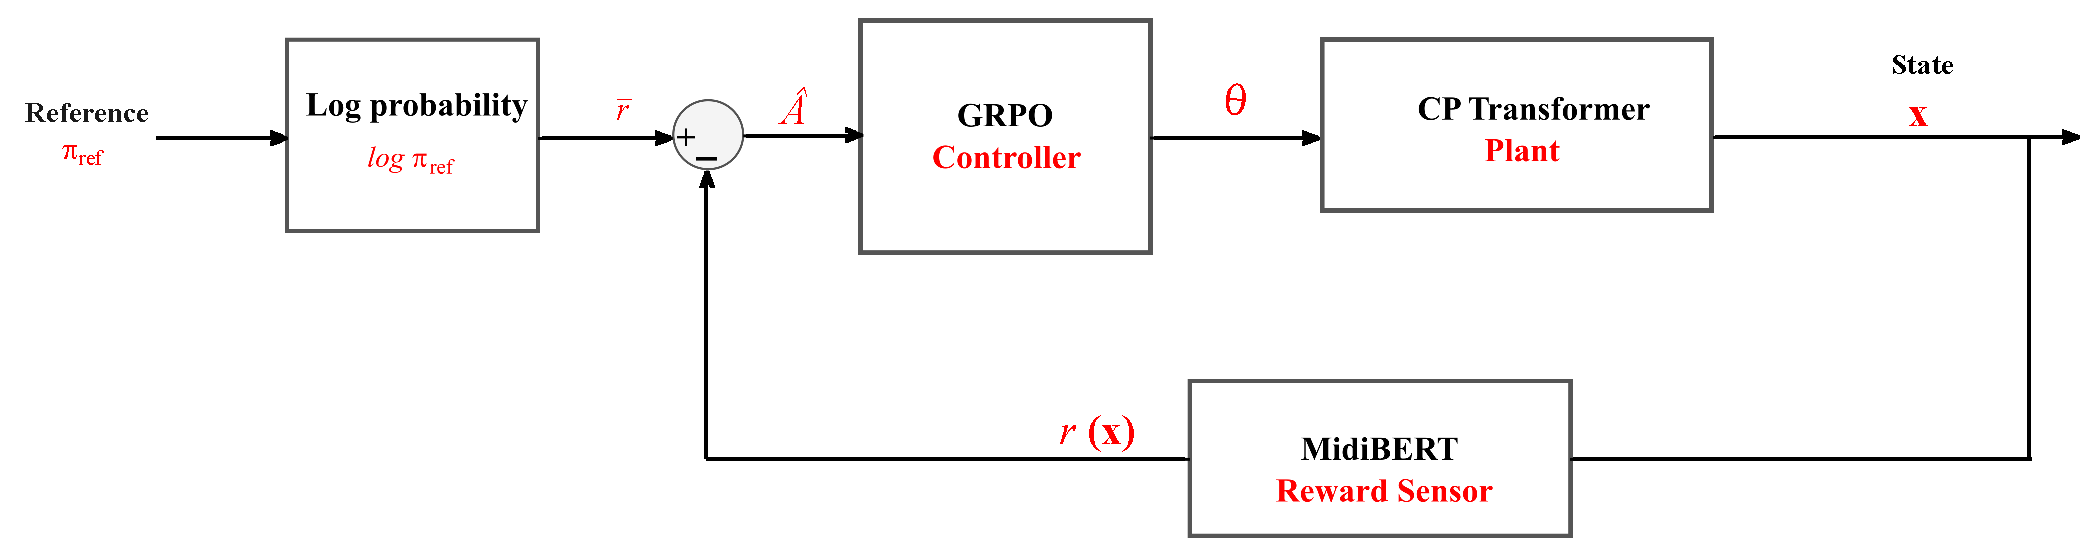
\includegraphics[width=0.7\linewidth]{figures/figBLOCK.eps}
\caption{Block diagram of the proposed closed-loop music generation scheme. The GRPO controller minimizes tracking error (group-relative advantage $\hat{A}$) between the plant output reward $r(\textbf{x})$ and the reference reward $\bar{r}$.}
\label{fig:block}
\end{figure*}
\par This motivates the present work, which integrates RL with control-theoretic principles for music generation. Specifically, this paper investigates the RL-based fine-tuning of music generation models within a feedback control framework using the group relative policy optimization (GRPO) \cite{shao2024deepseekmath} approach.
GRPO is a recently introduced RL algorithm whose application to music generation remains relatively unexplored. One of the existing studies in this direction is \cite{zhang2025}, which investigates lyric-to-song generation using RL preference optimization, demonstrating that GRPO can effectively reduce hallucinations while preserving musical quality. Beyond music generation, GRPO has also been successfully applied to other generative tasks. For example, \cite{xue2025} extends GRPO to image and video generation by aligning diffusion and flow-based generative models with human preferences, while \cite{liu2026} proposes a unified GRPO-based framework for reasoning-driven multimodal generation, jointly optimizing text and image generation policies. These studies highlight the growing potential of GRPO as a general RL framework for aligning generative models and human preferences across diverse modalities such as image, text, and audio. In the present work, GRPO is employed as a controller that learns an optimal policy for music generation. This provides a systematic framework for guiding the generation process toward desired musical objectives while improving long-term performance and stability.   The key elements of the proposed RL-based music generation scheme from a feedback-control perspective are summarized as follows (see Fig. \ref{fig:block}):
\begin{itemize}[leftmargin=*]
    \item \textbf{Plant:} A causal CP Transformer whose internal state is denoted by $\textbf{x}\in \mathbb{R}^{n},$ which evolves as a discrete-time dynamical system over compound-word tokens.
    \item \textbf{Sensor:} A pretrained MidiBERT encoder~\cite{midibertpiano} with a scalar reward head, providing a quality measurement $r(\textbf{x}) \in \mathbb{R}$ for each state $\textbf{x}\in \mathbb{R}^{n}$.
    \item \textbf{Reference signal:} A frozen copy of the pretrained policy $\pi_{\mathrm{ref}}$, whose log-probabilities define the desired reward reference $\bar{r}$.
    \item \textbf{Controller:} computes control updates using a GRPO-based policy that uses group-normalized advantages.
    \item \textbf{Stability constraint:} KL divergence between the active policy and the reference policy \cite{Jaques2016}, bounding the deviation from the pretrained equilibrium.
    \item \textbf{Entropy regularization:} An entropy floor term that prevents the policy from collapsing to a deterministic map.
\end{itemize}
Among the existing literature, the proposed approach is most closely related to the RL framework with KL regularization  \cite{Jaques2016}, the Transformer-based symbolic music generation  \cite{Huang2018}, and the model predictive control-based music generation  \cite{Augustine2025}. Compared with \cite{Jaques2016,Huang2018, Augustine2025}, the main contributions of this paper are as follows: (i) a control-theoretic formulation of RL-based music generation where the Transformer model acts as the plant with the GRPO as the controller; (ii) a complete implementation on the ATEPP classical piano dataset using a MidiBERT-based reward model as the sensor; and (iii) empirical validation that the resulting closed-loop system achieves reward improvement while maintaining bounded state drift.

\par The remainder of this paper is organized as follows. Section II provides an overview of the proposed closed-loop music generation scheme using a block diagram. Sections III–V describe its key components: the CP Transformer (plant model) in Section III, the MidiBERT-based reward sensor in Section IV, and the GRPO controller in Section V. Section VI presents the numerical implementation of the proposed approach and discusses the simulation results. Finally, Section VII concludes the paper and outlines directions for future research.

% ═══════════════════════════════════════════════════════════════
\section{System Architecture}

Fig.~\ref{fig:block} shows a block diagram of the proposed closed-loop music generation scheme. 
In this paper, the closed-loop policy is denoted by $\bm{\pi}_{\theta}$, which is parameterized by $\bm{\theta} \in \mathbb{R}^{n_{\theta}}$. Our approach directly learns a closed-loop dynamical system of the form: 
\begin{equation}
    \label{eq:generalmodel}
    \textbf{x}_{t+1}=\textbf{f}(\textbf{x}_{\leq t}; \bm{\pi}_{\bm{\theta}})
\end{equation}    
  using a Transformer-based model during the pretraining stage. Subsequently, the learned policy is further improved through a fine-tuning stage using the GRPO controller, enabling improved control performance.
At each GRPO iteration, the controller samples a batch of prompt states from the training set, generates multiple completions using the plant (CP Transformer), and evaluates them with a reward sensor (MidiBERT), which computes the reward value $r(\textbf{x})$. It then computes group-relative advantages $\hat{A}$ as an error signal and updates the parameters $\bm{\theta}$ using an RL objective function with a KL penalty (GRPO). 

% \begin{figure}[t]
% \centering
% \begin{tikzpicture}[
%     node distance=0.8cm and 0.6cm,
%     block/.style={rectangle, draw, rounded corners=2pt, minimum width=2.0cm, minimum height=0.6cm, align=center, font=\scriptsize, fill=#1},
%     block/.default={blue!8},
%     sum/.style={circle, draw, minimum size=0.4cm, inner sep=0pt, font=\scriptsize},
%     arrow/.style={-{Stealth[length=2mm]}, thick},
% ]
%     \node[block=green!10] (ref) {Reference\\$\bm{\pi}_{\mathrm{ref}}$};
%     \node[sum, right=0.7cm of ref] (sum) {$-$};
%     \node[block=orange!12, right=0.7cm of sum] (ctrl) {GRPO\\Controller};
%     \node[block=blue!10, right=0.7cm of ctrl] (plant) {CP Transformer\\(Plant)};
%     \node[block=red!10, below=0.8cm of plant] (sensor) {MidiBERT\\Reward Sensor};

%     \draw[arrow] (ref) -- (sum) node[midway, above, font=\scriptsize] {$\log \bm{\pi}_{\mathrm{ref}}$};
%     \draw[arrow] (sum) -- (ctrl) node[midway, above, font=\scriptsize] {$\hat{A}$};
%     \draw[arrow] (ctrl) -- (plant) node[midway, above, font=\scriptsize] {$\Delta\bm{\bm{\theta}}$};
%     \draw[]  (plant) -| ++(1.0,0) |- (sensor) node[near start, left, font=\scriptsize] {$\textbf{x}$};
%     \draw[arrow] (sensor) -| (sum) node[near start, below, font=\scriptsize] {$r(\textbf{x})$};
% \end{tikzpicture}
% \caption{Block diagram of closed-loop music generation scheme. The GRPO controller minimizes tracking error (group-relative advantage $\hat{A}$) between the plant output reward and the reference policy setpoint.}
% \label{fig:block}
% \end{figure}

% ═══════════════════════════════════════════════════════════════
\section{Plant Model: CP Transformer}

%\subsection{State-Space Representation}
The proposed Transformer-based music generator can be modeled as a discrete-time dynamical system. In this representation, time is indexed by discrete steps $t$, where each step corresponds to the generation of a single token in the output sequence. The system state at time $t$ is represented by a compound-word token, which encodes the relevant musical information at that step, denoted as:
\begin{equation}
    \textbf{x}_t = \bigl[\,x_{t}^{\mathrm{Bar}},\; x_{t}^{\mathrm{Pos}},\; x_{t}^{\mathrm{Pitch}},\; x_{t}^{\mathrm{Dur}}\,\bigr] \in \mathbb{X}
\end{equation}
where $\mathbb{X} = \mathbb{X}_{\mathrm{Bar}} \times \mathbb{X}_{\mathrm{Pos}} \times \mathbb{X}_{\mathrm{Pitch}} \times \mathbb{X}_{\mathrm{Dur}} \subseteq \mathbb{R}^{n}$ is the joint vocabulary carries simultaneous information about bar structure ($x_{t}^{\mathrm{Bar}}$), rhythmic position ($x_{t}^{\mathrm{Pos}}$), pitch ($x_{t}^{\mathrm{Pitch}}$), and duration ($x_{t}^{\mathrm{Dur}}$). Here $\mathbb{X}$ is a product of four discrete sets with  $|\mathbb{X}| = 4 \times 18 \times 90 \times 66$. This factored state space is central to the compound word representation~\cite{cp_representation}. The state transition is governed by the policy $\bm{\pi}_{\bm{\theta}}$ through a Transformer model as discussed next.  %{\color{cyan} Comment: Should it be $|\mathbb{X}|$ instead of $|\mathcal{V}|$? Also, should the state be represented using $\textbf{x}$ as in Fig. 1, instead of $\textbf{s}$?}.


% \begin{equation}
%     \textbf{x}_{t+1} \sim \bm{\pi}_{\bm{\theta}}(\cdot \mid \textbf{x}_{\le t})
% \end{equation}
%{\color{cyan}Comment: Is $\textbf{s}_{t+1}$ be $\bm{\pi}_{\bm{\theta}}$ itself or some function (denoting Transformer) of $\bm{\pi}_\bm{\theta}$?   }

%rather than flattening musical attributes into a single token stream, each time step.
\subsection{Transformer Architecture}
In this paper, a Transformer network \cite{Vaswani2017} is used to represent the plant model as in Eq. (\ref{eq:generalmodel}) and can be represented as
\begin{equation}
\label{eqNNTF}
\textbf{x}_{t+1} = \textbf{f}_{\text{TF}} (\textbf{X}_{t};\bm{\theta}) =  \textbf{f}_{\text{L}}\Big(\textbf{f}_{{\text{L-1}}}\big(\dots \textbf{f}_{1}(\textbf{X}_{t})\big)\Big)
\end{equation}
where $\text{L}$ is the number of Transformer layers and $\textbf{f}_{i}$, $i = 1, 2, \dots, \text{L}$, denotes the $i^{\text{th}}$ Transformer layer, $\bm{\theta}$ contains all parameters in the Transformer model. The matrix $\textbf{X}_{t}\in \mathbb{R}^{\text{N}\times n}$ contains $\text{N}$ samples of past state vectors, where the final row corresponds to $\textbf{x}_t$. Each Transformer layer consists of a sequential connection of two sub-networks, both equipped with residual connections: (i) a multi-head self-attention (MHSA) network, and (ii) a multi-layer perceptron (MLP) network \cite{Vaswani2017}. The MHSA stage consists of multiple self-attention operations applied in parallel, which can be represented as:
\begin{equation}
\label{eqfMHSA}
\textbf{f}_{\text{MHSA}} (\textbf{X}) = \sum_{i=1}^{\text{H}}  \textbf{A}_{a_{i}} \textbf{X} \textbf{W}_{\mathrm{proj}_{i}}
\end{equation}
where $\text{H}$ denotes the number of attention heads, $\textbf{A}_{a_{i}} \in \mathbb{R}^{\text{N} \times \text{N}}$ represents the attention matrix at $i^{th}$ head, and $\textbf{W}_{\mathrm{proj}_i}$ is the weight matrix of the $i^{th}$ head. %The plant is a causal Transformer with separate embedding tables per attribute, concatenation-projection input fusion, and independent linear prediction heads:
 %represented as: }
%\begin{equation}
%    \textbf{h}_t = \textbf{W}_{\mathrm{proj}} \bigl[\, E_{\mathrm{Bar}}(x_{t}^{\mathrm{Bar}}) \;\|\; \cdots \;\|\; E_{\mathrm{Dur}}(x_{t}^{\mathrm{Dur}}) \,\bigr]
%\end{equation}
The MHSA block is followed by an MLP block, which contains $\mathrm{M}$ hidden layers. The Transformer parameter vector $\bm{\theta}$ consists of the parameters of the MHSA network and the MLP network.
Table~\ref{tab:plant} summarizes the Transformer dimensions and number of parameters.

\begin{table}[t!]
\centering
\caption{Plant (CP Transformer) configuration}
\label{tab:plant}
\begin{tabular}{@{}lr@{}}
\toprule
\textbf{Parameter} & \textbf{Value} \\
\midrule
Hidden dimension $d$ & 512 \\
Transformer layers $\text{L}$ & 8 \\
Attention heads $\text{H}$ & 8 \\
Feed-forward dimension & 2048 \\
Attribute embedding dim & 128 \\
Max sequence length $T$ & 512 \\
Total parameters & ${\sim}26$M \\
Trainable fraction (GRPO) & 100\% \\
\bottomrule
\end{tabular}
\end{table}

%\subsection{Pretraining as System Identification}
\par Transformer model training is performed via MLE on the ATEPP corpus~\cite{atepp}, where the Transformer parameter vector  $\bm{\theta}$ is optimized to maximize the likelihood of the observed data.
The training objective is the standard next-token cross-entropy loss computed over all four attribute heads, resulting in the following loss function:
\begin{equation}
    \mathcal{L}_{\mathrm{TF}} = -\sum_{t=1}^{T}  \log p_{\bm{\theta}}\bigl(\textbf{x}_{t} \mid \textbf{x}_{<t}\bigr).
\end{equation}
%where $\mathcal{K} = \{\mathrm{Bar}, \mathrm{Pos}, \mathrm{Pitch}, \mathrm{Dur}\}$.
We train for 100 epochs on the 75 $\%$ pretraining split (approximately 10,500 sequences of length 512), using the AdamW optimizer with cosine annealing, decaying the learning rate from $3 \times 10^{-4}$ to nearly zero. The held-out evaluation loss decreases monotonically from $6.02$ to $4.02$ over approximately 54,000 gradient steps.
% ═══════════════════════════════════════════════════════════════
\section{Reward Sensor: MidiBERT}

\subsection{Sensor Architecture}

The reward sensor is used to evaluate the quality of the musical score generated, and it maps a CP sequence $\textbf{x}$ to a scalar quality score $r(\textbf{x})$. The reward sensor is defined using MidiBERT-Piano~\cite{midibertpiano}, which is a 12-layer bidirectional Transformer pretrained with masked language modeling on symbolic music data. A reward head is then appended to the model to compute the reward value corresponding to the state vector:
\begin{equation}
\label{eq_sensor}
    r(\textbf{x}) = \mathrm{MLP}\bigl(\mathrm{MeanPool}(\mathrm{MidiBERT}(\textbf{x}))\bigr) \in \mathbb{R}.
\end{equation}
The MLP dimensions are $768 \to 256 \to 64 \to 1$ with Gaussian error linear unit (GELU) activations, optimized by Optuna hyperparameter search~\cite{optuna}.

\subsection{Sensor Calibration via Bradley--Terry}

The reward sensor model in Eq. (\ref{eq_sensor}) is trained using synthetic preference pairs derived from the MAESTRO dataset~\cite{maestro}. To construct these pairs, five corruption strategies: bar shuffling, pitch randomization, position jitter, note dropout, and duration noise, are applied to ground-truth sequences to generate corrupted versions. Pairing each corrupted sequence with its corresponding original sequence ensures that both samples share the same source, thereby eliminating confounding stylistic variations and allowing the comparison to focus solely on the introduced corruptions. The sensor calibration loss follows the Bradley--Terry ranking model~\cite{bradley1952rank}:
\begin{equation}
    \mathcal{L}_{\mathrm{sensor}} = -\mathbb{E}\bigl[\log \sigma\bigl(r(\textbf{x}^w) - r(\textbf{x}^l) - m\bigr)\bigr]
\end{equation}
where $m = 1.0$ is a margin ensuring reward separation.

Parameter efficiency is achieved through low-rank adaptation~\cite{hu2022lora} with rank $r = 8$ and scaling factor $\alpha = 16$, applied to the last four attention layers. This setup results in approximately $0.28\%$ trainable parameters.
During GRPO training, the sensor term is kept frozen, and its parameters are not updated. As a result, it operates as a fixed measurement instrument throughout the optimization process.

% ═══════════════════════════════════════════════════════════════
\section{Controller Design: GRPO}



\subsection{Control Law}

At each control step, the GRPO controller begins by sampling a batch of $B$ prompt states from the fine-tuning split. For each prompt, it generates $G$ completions using nucleus sampling, resulting in grouped rollouts. All $B\times G$ generated completions are then evaluated using the reward sensor to obtain their corresponding reward values. Next, group-relative advantages are computed by normalizing the rewards within each prompt group as follows:
    \begin{equation}
        \hat{A}_{i,g} = \frac{r_{i,g} - \bar{r}_i}{\sigma_{r_i} + \epsilon}.
    \end{equation}
    Finally, the GRPO loss is defined using a clipped surrogate objective that includes a KL divergence penalty as in \cite{Jaques2016} and an entropy regularization term \cite{Jaques2016,haarnoja2018}, resulting in:
    \begin{equation}
    \label{eq_L_GRPO}
    \begin{split}
        \mathcal{L}_{\mathrm{GRPO}} = -\mathbb{E}\bigl[\min\bigl(\rho \hat{A},\; \mathrm{clip}(\rho, 1{\pm}\varepsilon)\hat{A}\bigr)\bigr] \\
        + \beta \, D_{\mathrm{KL}}\!\bigl(\bm{\pi}_{\bm{\theta}} \| \bm{\pi}_{\mathrm{ref}}\bigr) + \lambda \, \mathcal{P}_{\mathrm{ent}}
    \end{split}
    \end{equation}
where $D_{\mathrm{KL}}(\bm{\pi}_{\bm{\theta}} \| \bm{\pi}_{\mathrm{ref}})$ is the KL divergence term which measures the divergence between the current policy $\bm{\pi}_{\bm{\theta}}$ and reference policy $\bm{\pi}_{\mathrm{ref}},$
$\rho = \bm{\pi}_{\bm{\theta}} / \bm{\pi}_{\mathrm{old}}$ is the importance ratio, $\varepsilon = 0.2$ is the clip range, $\beta = 0.03$ is the KL coefficient, and $\lambda = 0.02$ weights the entropy penalty $\mathcal{P}_{\mathrm{ent}}.$  
Here the entropy penalty $\mathcal{P}_{\mathrm{ent}}$ is used to enhance randomness and is defined as:
\begin{equation}
    \mathcal{P}_{\mathrm{ent}} = \max\bigl(0,\; H_{\mathrm{target}} - \bar{H}_{\mathrm{norm}}\bigr)^2
\end{equation}
where $\bar{H}_{\mathrm{norm}}$ is the normalized completion entropy averaged over CP attributes and $H_{\mathrm{target}} = 0.55$ is the minimum acceptable entropy. 
A policy that collapses toward near-deterministic sampling loses the capacity to explore alternative trajectories, thereby significantly reducing its exploratory diversity. From a control-theoretic perspective, this is equivalent to a loss of effective controllability: the control input (i.e., the GRPO gradient update) can no longer meaningfully steer or reshape the output distribution. As a result, the system becomes constrained to a narrow subset of the state-space, limiting its responsiveness to optimization signals and reducing its ability to adapt to alternative high-reward regions of the policy space.

\par In the GRPO controller, the RL policy parameters are updated in the direction that minimizes the GRPO loss.  The resulting GRPO control law becomes:
\begin{equation}
    \label{GRPO_control}
    \bm{\pi}_{\bm{\theta}}^{*}=\underset{\bm{\pi}_{\bm{\theta}}}{\arg \min} \hspace{.2cm}  \mathcal{L}_{\mathrm{GRPO}}.
\end{equation} 
The learning rate for the GRPO controller is scheduled using cosine annealing, decreasing from $7.5 \times 10^{-6}$ to $7.5 \times 10^{-7}$ over 1500 steps. From a control-theoretic perspective, this can be interpreted as a form of gain scheduling, where the optimization begins with relatively large update steps (high gain) to enable rapid initial learning and gradually transitions to smaller, more stable updates (low gain) for fine refinement. This behavior is analogous to switching from a fast-response controller during transient phases to a precision controller as the system approaches steady state. Table~\ref{tab:grpo} summarizes the GRPO controller configuration.

\begin{table}[t]
\centering
\caption{GRPO controller hyperparameters}
\label{tab:grpo}
\begin{tabular}{@{}lr@{}}
\toprule
\textbf{Parameter} & \textbf{Value} \\
\midrule
Total control steps & 1500 \\
Batch size $B$ & 2 \\
Group size $G$ & 6 \\
Prompt length & 64 tokens \\
Completion length & 128 tokens \\
Clip range $\varepsilon$ & 0.2 \\
KL coefficient $\beta$ & 0.03 \\
Entropy coefficient $\lambda$ & 0.02 \\
Entropy target $H_{\mathrm{target}}$ & 0.55 \\
Learning rate (initial) & $7.5 \times 10^{-6}$ \\
LR schedule & Cosine annealing \\
Gradient clipping & 1.0 \\
\bottomrule
\end{tabular}
\end{table}

\subsection{Stability via KL Regularization}

In this section, we informally discuss the stability of the GRPO controller using the Lyapunov approach \cite{Lyapunov1892,Khalil2002,Michel2015}. To this end, we consider the KL divergence penalty term in Eq. (\ref{eq_L_GRPO}) as a candidate Lyapunov function $V(\bm{\theta}) = D_{\mathrm{KL}}(\bm{\pi}_{\bm{\theta}} \| \bm{\pi}_{\mathrm{ref}})$.  This selection quantifies the extent of deviation from the reference policy and attains its minimum value when the two policies coincide. Since the KL divergence is nonnegative and $D_{\mathrm{KL}}(\bm{\pi}_{\bm{\theta}}\| \bm{\pi}_{\mathrm{ref}})=0$ at $\bm{\pi}_{\bm{\theta}}=\bm{\pi}_{\mathrm{ref}},$ we have $V(\bm{\theta}) \geq 0$ and $V(\bm{\theta})=0,$ at $\bm{\pi}_{\bm{\theta}}=\bm{\pi}_{\mathrm{ref}}.$ 
The GRPO update with KL penalty coefficient $\beta > 0$ results in:
\begin{equation}
    \Delta V \le \frac{1}{\beta}\bigl(\mathcal{L}_{\mathrm{GRPO}} - \mathcal{L}_{\mathrm{GRPO}}^*\bigr).
\end{equation}
Now, at the global optima, we have $\mathcal{L}=\mathcal{L}^{*}$ which results in $\Delta V \leq 0.$ This indicates that $V(\bm{\theta})$ can serve as a Lyapunov function, and the resulting closed-loop system under the GRPO controller is Lyapunov stable (see Theorem 4.1 in \cite{Khalil2002}). 
In addition, the clipping mechanism enforces the constraint $|\rho - 1| \le \varepsilon$, which can be interpreted as an actuator saturation effect that limits the magnitude of per-step policy updates and, consequently, restricts abrupt changes in the state transitions. Taken together, the KL penalty and the clipping operation define an implicit trust region around the reference policy. This trust region ensures that the updated policy remains within a bounded neighborhood of the reference equilibrium, thereby promoting stable and controlled policy evolution across iterations. This is directly analogous to gain-limited control where the controller cannot drive the plant arbitrarily far from its identified operating point in a single step. 

% ═══════════════════════════════════════════════════════════════
\section{Experimental Setup and Results}

%\subsection{Dataset}

The ATEPP dataset~\cite{atepp}, consisting of approximately 14,000 sequences of classical piano performances, is used for training and validation. After CP tokenization with a sequence length of 512 and deterministic splitting (seed 52), the dataset is partitioned into two subsets. The pretraining split (75\%) contains approximately ${\sim}10{,}500$ sequences and is used for CP Transformer identification, while the GRPO split (25\%) contains approximately ${\sim}3{,}500$ sequences and is reserved for closed-loop fine-tuning with GRPO.

%\subsection{Training Pipeline}

The training consists of two phases. In Phase 1 (Transformer pretraining), the model is trained for 100 epochs with a batch size of 128 using the AdamW optimizer (learning rate = $3 \times 10^{-4}$) and a cosine learning rate schedule. Mixed-precision training is employed, resulting in approximately ${\sim}54{,}000$ optimization steps.
In Phase 2 (fine-tuning with GRPO), the closed-loop performance is further optimized for 1500 steps using the frozen MidiBERT reward sensor and the complementary 25\% data split. The best checkpoint obtained from pretraining is used to initialize both the active policy network and the frozen reference model.
% ═══════════════════════════════════════════════════════════════
%\section{Results and Analysis}

\subsection{Transformer Model Pretraining}

Fig.~\ref{fig:pretrain} illustrates the pretraining loss trajectory.
The training loss decreases from $7.39$ (epoch 1) to $3.38$ (epoch 62), while the evaluation loss decreases from $6.02$ to $4.01$.
The monotonic decrease without divergence confirms that the model identification is well-conditioned.
The gap between training and evaluation loss (${\sim}0.6$ at convergence) indicates mild overfitting, acceptable for a model that will be further refined by the GRPO controller.

\begin{figure}[h!]
\centering
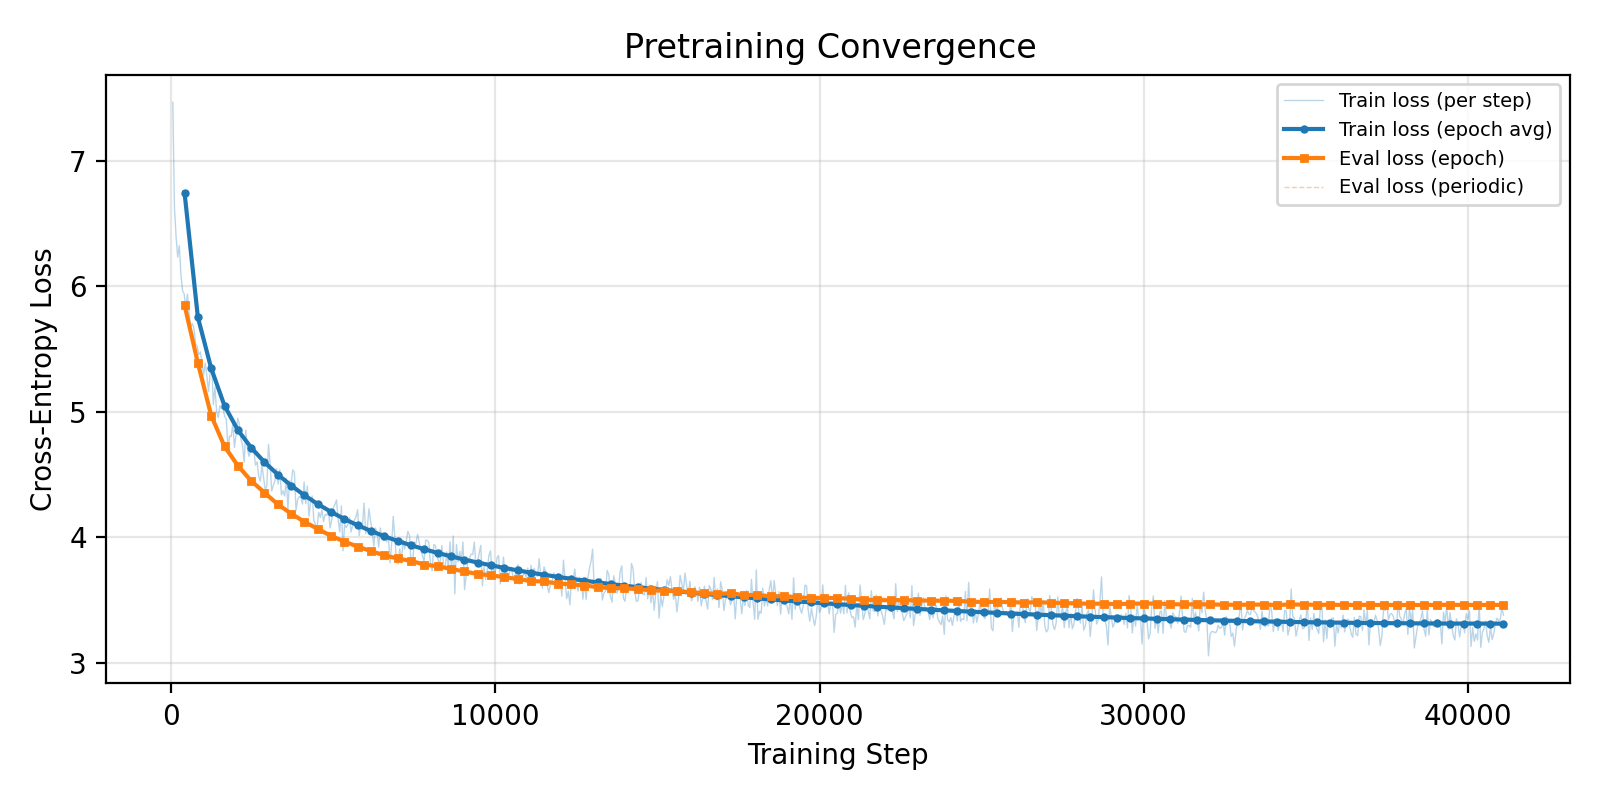
\includegraphics[width=1\linewidth]{figures/pretrain_loss_curve.png}
\caption{Pretraining loss values over 40000 training steps.}
\label{fig:pretrain}
\end{figure}
\subsection{Fine-tuning with GRPO Controller}
The pretrained Transformer model is subsequently fine-tuned using the GRPO controller. Figure~\ref{fig:reward} illustrates the evolution of the reward function over 1,500 GRPO training steps. Table~\ref{tab:reward_evolution} summarizes the evaluation reward at selected GRPO checkpoints. 
 The mean evaluation reward improves from $-10.61$ at step~100 to $+2.53$ at step~1500, a net improvement of $+13.14$ reward units.
The improvement is most rapid during the first 500 steps (high-gain regime of the cosine schedule), consistent with the gain-scheduling interpretation. The normalized entropy in the GRPO metrics (reported by the controller) provides a direct measure of policy controllability.
Values consistently above the $H_{\mathrm{target}} = 0.55$ floor indicate that the policy retains sufficient stochasticity for exploration, confirming that the entropy penalty successfully prevents controllability loss.


\begin{figure}[h!]
\centering
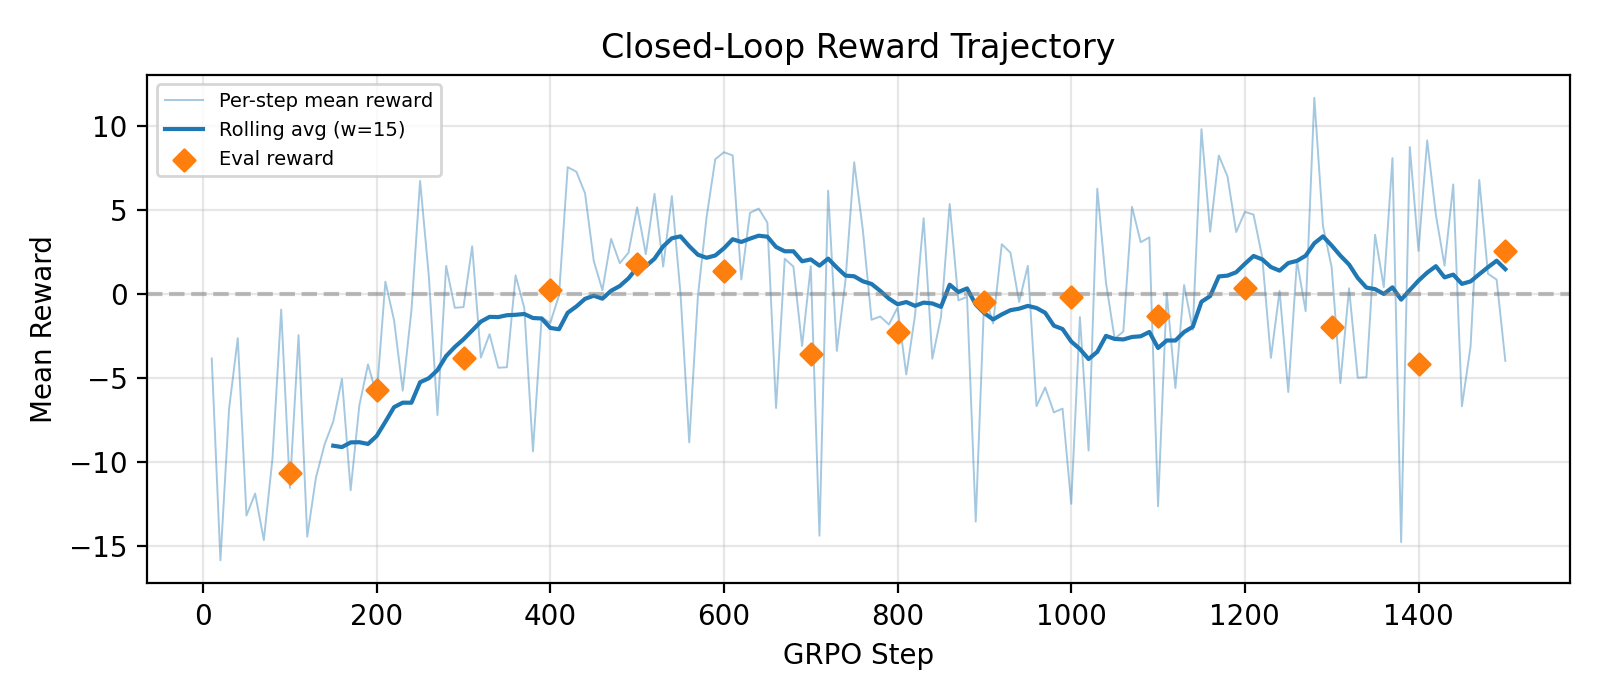
\includegraphics[width=1\linewidth]{figures/fig_reward.png}
\caption{Reward function values over 1500 GRPO steps.}
\label{fig:reward}
\end{figure}

\begin{table}[t]
\centering
\caption{Evaluation reward trajectory during GRPO}
\label{tab:reward_evolution}
\begin{tabular}{@{}rrrr@{}}
\toprule
\textbf{Step} & \textbf{Mean Reward} & \textbf{Std} & \textbf{Max} \\
\midrule
100 & $-10.61$ & 8.09 & 5.40 \\
200 & $-5.71$ & 7.95 & 7.59 \\
300 & $-3.83$ & 7.99 & 11.85 \\
400 & $+0.24$ & 8.03 & 12.41 \\
500 & $+1.78$ & 6.97 & 12.56 \\
600 & $+1.37$ & 9.03 & 16.97 \\
1000 & $-0.20$ & 11.44 & 14.68 \\
1500 & $+2.53$ & 10.09 & 17.26 \\
\bottomrule
\end{tabular}
\end{table}
%\subsection{Stability Analysis: KL Divergence}

\par The approximate KL divergence between the active policy and the reference policy increases from approximately ($10^{-6}$) at training step 10 to approximately (0.23) at step 1500, as shown in Fig. \ref{fig:kl}. This gradual, sub-linear increase indicates that the combined effect of the KL regularization term and the clipping mechanism effectively constrains policy updates, thereby maintaining the policy within a bounded neighborhood of the reference policy. These observations provide empirical support for the Lyapunov-based stability argument presented in Section~V-B. Furthermore, the clip fraction remains equal to zero throughout the training process, indicating that the clipping constraint is never activated. This suggests that, for the selected regularization coefficient ($\beta = 0.03$), the KL penalty alone is sufficient to preserve trust-region stability and prevent excessive policy deviations. Consequently, the clipping mechanism primarily serves as a safeguard against potentially large updates rather than acting as the principal stabilizing component of the optimization process.



\begin{figure}[h!]
\centering
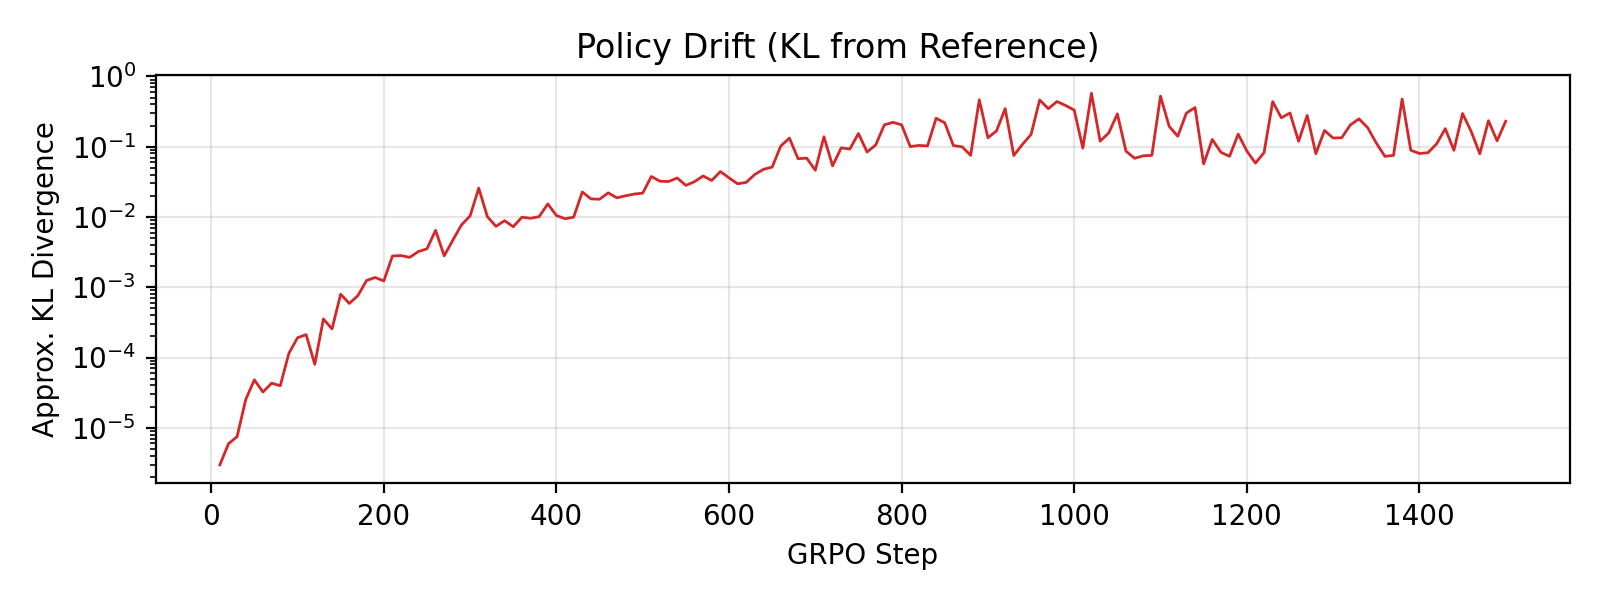
\includegraphics[width=\linewidth]{figures/fig_kl.png}
\caption{KL divergence loss over 1500 GRPO steps}
\label{fig:kl}
\end{figure}


%\subsection{Discussion}

\par The relatively high variance in the per-step reward ($\sigma \approx 4-13$) is primarily due to the stochastic nature of nucleus sampling and the small batch size ($B = 2$, $G = 6$). From a control-theoretic perspective, this behavior is similar to a system affected by process noise, resulting in noticeable short-term fluctuations. The evaluation rewards, which are computed using larger batches, exhibit a smoother and more consistent upward trend because the effects of random variations are averaged out. As a result, they provide a clearer view of the overall learning progress. The reward does not increase at every training step, which is expected. The clipped surrogate objective with KL regularization prioritizes stable policy updates rather than maximizing reward at each iteration. In addition, the cosine learning-rate schedule gradually reduces the update magnitude as training progresses. Despite these fluctuations, the overall increase in reward demonstrates that the policy is being effectively guided toward improved performance while maintaining stable learning dynamics.
% ═══════════════════════════════════════════════════════════════
\section{Conclusion}

This paper presented a control-theoretic framework for RL-based symbolic music generation by modeling the CP Transformer as a discrete-time plant, the MidiBERT reward model as a calibrated sensor, and GRPO as a feedback controller. Experimental results on the ATEPP dataset demonstrate the effectiveness of the proposed approach, with Transformer pretraining converging to an evaluation loss of 4.01 after 54K steps and GRPO improving the mean evaluation reward by 13.14 units over 1,500 optimization steps. Throughout training, the KL divergence remained below 0.25, indicating stable trust-region behavior, while the policy entropy stayed above the minimum threshold, preventing policy collapse. Future work will investigate adaptive KL scheduling for improved training dynamics, multi-objective reward design to enforce additional musical constraints, and robustness analysis under reward model uncertainty to establish connections with $H_\infty$ control.


% This paper presented a control-theoretic formulation for RL-based symbolic music generation by modeling the CP Transformer generator as a discrete-time plant, the MidiBERT reward model as a calibrated sensor, and the GRPO as a feedback controller. Experimental evaluation on the ATEPP dataset demonstrated the effectiveness of the proposed framework. The Transformer pretraining stage converged to an evaluation loss of 4.01 after 54K training steps, while the closed-loop GRPO optimization improved the mean evaluation reward by 13.14 units over 1,500 control steps. Furthermore, the KL divergence remained bounded below 0.25 throughout training, indicating stable trust-region behavior, and the policy entropy consistently exceeded the minimum acceptable threshold, thereby avoiding policy collapse. These results demonstrate that interpreting RL-based music generation within a feedback control framework provides a principled perspective for analyzing training dynamics and policy stability. Future work will investigate adaptive KL scheduling inspired by variable-structure control to improve transient response during policy optimization. In addition, extending the reward formulation to a multi-objective framework will enable the simultaneous enforcement of musical constraints such as harmonic consonance and rhythmic regularity, naturally leading to a multiple-input multi-output control formulation. Finally, robustness analysis under reward model uncertainty will be explored to establish theoretical connections with $H_\infty$ control and to improve the reliability of RL-based symbolic music generation.

% ═══════════════════════════════════════════════════════════════
\begin{thebibliography}{12}

\bibitem{Nierhaus2009}
G.  Nierhaus, \emph{Algorithmic Composition: Paradigms of Automated Music Generation}, Springer Vienna, 2009.

\bibitem{Yu2026}
D. Yu, K. Lee, and Y. Huang, \textquotedblleft  Generative modeling of bach-style symbolic music: A comparative study of autoregressive, latent-variable, and adversarial approaches," \emph{arXiv preprint}, 2026.






\bibitem{Allan2004}
M. Allan and C. Williams, \textquotedblleft  Harmonising chorales by probabilistic inference,"  \emph{17$^{th}$ Conference on Neural Information Processing Systems}, Vancouver, Canada, 2004.

\bibitem{Boenn2010}
G. Boenn, M. Brain, M. Vos, and J. Ffitch, \textquotedblleft  Automatic music composition using answer set programming," \emph{arXiv preprint}, 2010.

\bibitem{Anders2012}
T. Anders and E. Miranda, \textquotedblleft  Constraint programming systems for modeling music theories and composition
," \emph{ACM Computing Surveys}, vol. 43, pp. 1-38, 2012.

\bibitem{Briot2020}
J. Briot, G. Hadjeres, and F. Pachet, \emph{Deep Learning Techniques for
Music Generation}, Springer, 
 2020.

 \bibitem{Loy2006}
G. Loy, \emph{Musimathics: The Mathematical Foundations of Music, Volume 1}, MIT Press, 
 2006.

 \bibitem{Astrom2008}
K. Astrom and
R. Murray, \emph{Feedback Systems; An Introduction for Scientists and Engineers},   Princeton University Press, 
 2008.
 
 \bibitem{holtzman2020curious}
A.~Holtzman, J.~Buys, L.~Du, M.~Forbes, and Y.~Choi,
``The curious case of neural text degeneration,''
\emph{International Conference on Learning Representations}, 2020.
  \bibitem{Jaques2016}
N. Jaques, S. Gu, D. Bahdanau, J. Lobato, R. Turner, and D. Eck, \textquotedblleft Sequence tutor: Conservative fine-tuning of sequence generation models with KL-control," \emph{arXiv preprint}, 
 2016.


\bibitem{Kotecha2018}
N. Kotecha,
``Bach2Bach: Generating music using a deep reinforcement learning approach
,''
\emph{arXiv preprint}, 2018.

\bibitem{dadman2023}
S. Dadman and B. Bremdal,
``Multi-agent reinforcement learning for structured symbolic music generation,''
\emph{Advances in Practical Applications of Agents, Multi-Agent Systems, and Cognitive Mimetics}, Springer, vol. 13955, pp. 52--63,  2023.

\bibitem{dadman2024}
S. Dadman and B. Bremdal,
``Crafting creative melodies: A user-centric approach for symbolic music generation,''
\emph{Electronics}, vol. 13, no. 6, 2024.

\bibitem{cideron2024}
G. Cideron, S. Girgin, M. Verzetti, D. Vincent, M. Kastelic, Z. Borsos, B. McWilliams, V. Ungureanu, O. Bachem, O. Pietquin, M. Geist, L. Hussenot, N. Zeghidour,  and A. Agostinelli, 
``MusicRL: Aligning music generation to human preferences,''
\emph{arXiv preprint}, 2024.

 \bibitem{Justus2023}
A. Justus, \textquotedblleft Music generation using human-in-the-loop RL," \emph{ IEEE International Conference on Big Data}, Sorrento, Italy,  
 2023.

 

\bibitem{Huang2018}
C. Huang, A. Vaswani, J. Uszkoreit, N. Shazeer, I. Simon, C. Hawthorne, A. Dai, M. Hoffman, M. Dinculescu, and D. Eck,
``Music Transformer,''
\emph{arXiv preprint}, 2018.


\bibitem{Ens2020}
J. Ens and P. Pasquier,
``MMM : Exploring conditional multi-track music generation with the Transformer
,''
\emph{arXiv preprint}, 2020.

\bibitem{Shih2022}
Y. Shih, S. Wu, F. Zalkow; M. Muller, and Y. Yang,
``Theme Transformer: Symbolic music generation with theme-conditioned Transformer
,''
\emph{IEEE Transactions on Multimedia}, vol. 25, 2022.

\bibitem{Yu2022}
C. Yu, P. Lu, R. Wang, W. Hu, X. Tan, W. Ye, S. Zhang, T. Qin, and T. Liu,
``Museformer: Transformer with fine- and coarse-grained attention for music generation
,''
\emph{arXiv preprint}, 2022.

\bibitem{Wu2023}
S. Wu, X. Li, F. Yu, and M. Sun,
``TunesFormer: Forming Irish tunes with control codes by bar patching
,''
\emph{arXiv preprint}, 2023.

\bibitem{Copet2024}
J. Copet, F. Kreuk, I. Gat, T. Remez, D. Kant, G. Synnaeve, Y. Adi, and A. Defossez,
``Simple and controllable music generation
,''
\emph{arXiv preprint}, 2024.



\bibitem{shao2024deepseekmath}
 Z. Shao, P. Wang, Q. Zhu, R. Xu, J. Song, X. Bi, H. Zhang, M. Zhang, Y. Li, Y. Wu, and D. Guo,
``DeepSeekMath: Pushing the limits of mathematical reasoning in open language models,''
\emph{arXiv preprint}, 2024.

 \bibitem{zhang2025}
H. Zhang, W. Tan, G. Li, Y. Zhang, H. Chen, S. Lei, C. Yang,
Z. Wu, S. Wang, Q. Huang, and D. Yu,
``Towards hallucination-free music: A reinforcement learning preference optimization framework for reliable song generation,''
\emph{arXiv preprint}, 2025.


\bibitem{xue2025}
Z. Xue, J. Wu, Y. Gao, F. Kong, L. Zhu, M. Chen, Z. Liu, W. Liu, Q. Guo, W. Huang, and P. Luo,
``DanceGRPO: Unleashing GRPO on visual generation,''
\emph{arXiv preprint}, 2025.

\bibitem{liu2026}
J. Liu, Z. Ye, L. Yuan, S. Zhu, Y. Gao, J. Wu, K. Li, X. Wang, X. Nie, W. Huang, and W. Ouyang,
``UniGRPO: Unified policy optimization for reasoning-driven visual generation,''
\emph{arXiv preprint}, 2026.


\bibitem{midibertpiano}
Y.~Chou, I.~Chen, C.~Chang, J.~Ching, and Y.~Yang,
``MidiBERT-Piano: Large-scale Pre-training for Symbolic Music Classification Tasks,''
\emph{Journal of Creative Music Systems}, vol. 8, no. 1, 2024.

\bibitem{Augustine2025}
M. Augustine,
``Predictive controlled music,''
\emph{arXiv preprint}, 2025.

\bibitem{haarnoja2018}
T. Haarnoja, A. Zhou, P. Abbeel, and S. Levine,
``Soft actor-critic: Off-policy maximum entropy deep reinforcement learning with a stochastic actor,''
 \emph{ $35^{th}$ International Conference on Machine Learning}, Stockholm, Sweden, 2018.
% Widely used entropy/KL-regularized RL algorithm.

\bibitem{cp_representation}
W.~Hsiao, J.~Liu, Y.~Yeh, and Y.~Yang,
``Compound word Transformer: Learning to compose full-song music over dynamic directed hypergraphs,''
\emph{AAAI Conference on Artificial Intelligence}, 2021.


\bibitem{Vaswani2017} A. Vaswani, N. Shazeer, N. Parmar, J. Uszkoreit, L. Jones, A. Gomez, L. Kaiser, and I. Polosukhin, \emph{\textquotedblleft Attention is all you need,\textquotedblright}   
  $31^{st}$ Conference on Neural Information Processing Systems, Long Beach, U.S.A., 2017.

\bibitem{schulman2017ppo}
J.~Schulman, F.~Wolski, P.~Dhariwal, A.~Radford, and O.~Klimov,
``Proximal policy optimization algorithms,''
\emph{arXiv preprint}, 2017.



\bibitem{hu2022lora}
E. Hu, Y. Shen, P. Wallis, Z. Zhu, Y. Li, S. Wang, L. Wang, and W. Chen,
``LoRA: Low-rank adaptation of large language models,''
\emph{International Conference on Learning Representations}, 2022.

\bibitem{maestro}
C. Hawthorne, A. Stasyuk, A. Roberts, I. Simon, C. Huang, S. Dieleman, E. Elsen, J. Engel, and D. Eck,
``Enabling factorized piano music modeling and generation with the MAESTRO dataset,''
\emph{International Conference on Learning Representations}, New Orleans, U.S.A., 2019.


\bibitem{bradley1952rank}
R.~Bradley and M.~Terry,
``Rank analysis of incomplete block designs: I. The method of paired comparisons,''
\emph{Biometrika}, vol.~39, no.~3/4, pp.~324--345, 1952.



\bibitem{atepp}
H.~Zhang, J.~Tang, S.~Rafee, S.~Dixon, and G.~Fazekas,
``ATEPP: A dataset of automatically transcribed expressive piano performance,''
\emph{ $23^{rd}$ International Society for Music Information Retrieval Conference}, Bengaluru, India, 2022.

\bibitem{optuna}
T.~Akiba, S.~Sano, T.~Yanase, T.~Ohta, and M.~Koyama,
``Optuna: A next-generation hyperparameter optimization framework,''
\emph{$25^{th}$ ACM SIGKDD International Conference on Knowledge Discovery $\&$ Data Mining}, Anchorage, U.S.A., 2019.


\bibitem{mroueh2025}
Y. Mroueh, N. Dupuis, B. Belgodere, A. Nitsure, M. Rigotti, K. Greenewald, J. Navratil, J. Ross, and J. Rios,
``Revisiting group relative policy optimization: Insights into on-policy and off-policy training,''
\emph{arXiv preprint}, 2025.


\bibitem{Lyapunov1892} A. Lyapunov,
\emph{The General Problem of the Stability of Motion}.
Kharkov Mathematical Society, 1892.

\bibitem{Khalil2002}
H. Khalil, \textit{Nonlinear Systems}, 3rd Ed. Prentice Hall, 2002.

\bibitem{Michel2015}
A. Michel, L. Hou, and D Liu, \textit{Stability of Dynamical Systems;
On the Role of Monotonic and Non-Monotonic Lyapunov Functions, Second edition},  Springer,  2015.


\end{thebibliography}

\end{document}
